\chapter{Background}
\label{chap:background}

\section{Compartmental Models for the Spread of Infectious Disease}
\label{sec:outbreak_models}

Compartmental epidemic models are used to describe the dynamics of an outbreak, to estimate how features of the population or environment affect its severity, and to understand how interventions might help to disrupt transmission. A compartmental model represents the time--evolution of an outbreak in terms of the disease histories of individuals as they transition between discrete states, or model compartments. When we use a compartmental model to describe the \textit{transmission} dynamics of an outbreak, the model compartments encode structural information about how individuals at different infection states interact to transmit the infectious agent. In contrast, states in a compartmental model for \textit{disease} dynamics typically correspond to discrete stages in the natural history of within--host disease progression without reference to the host's transmissive potential. This distinction is diagrammed in Figure \ref{fig:infec_vs_disease}.

Mechanistic compartmental models prescribe physical laws that govern the transmission dynamics of an outbreak. For example, the model might specify the rates of infectious contact between groups of people, or with an environmental reservoir that is a vector for transmission. Infection incidence and prevalence data are modeled conditionally on the mechanistic structure of the model, which specifies a functional form for the temporal and spatial evolution of the epidemic process. In contrast with their mechanistic counterparts, phenomenological models describe the data generating mechanism without explicit reference to the physical system that is under observation \cite{chowell2017fitting}. The price we pay for adopting a mechanistic approach is that our models will be obviously ``wrong", at least in the sense that all models are wrong, so it will be our responsibility to justifying their reasonableness. Our reward is that mechanistic models provide us with interpretable, multifaceted descriptions of outbreak dynamics. Moreover, the ubiquity of mechanistic models in the epidemiological literature enables us to incorporate information about specific aspects of transmission dynamics from other studies and settings into our own models. Historical overviews of mechanistic models for disease transmission may be found in \cite{anderson1992infectious,brauer2017mathematical,keeling2008,lessler2016mechanistic}.

Mechanistic compartmental models can be specified at varying levels of fidelity to the underlying epidemic process. Our models will range in granularity, from agent--based models in which we explicitly track the disease histories of individuals, to population--level models defined by the aggregate flow of individuals between model compartments. All of the models in this work will treat the epidemic process as evolving continuously in time, but observed at discrete times. The decision to work with continuous--time models is advantageous when observation times are not evenly spaced, or when various sub--processes evolve on different time scales \cite{glass2003,shelton2014}. Discrete--time models can be problematic when the epidemic and observation processes are misaligned, and do not necessarily produce results that are independent of the choice time--step (see \cite{shelton2014} for examples). One (very) compelling reason to prefer discrete--time models is that the computational effort required to fit them is typically much lower than what is required in the continuous--time setting. 

\subsection{An Individual Level Susceptible--Infected--Recovered Model}
\label{subsec:sir_basics}
For clarity of exposition, we will contextualize the technical background on epidemic models in terms of the susceptible--infected--recovered (SIR model). Formal treatments that deal with this material in greater generality can be found in \cite{andersson2000stochastic,britton2018,brauer2008compartmental,fuchs2013inference,wilkinson2011stochastic}. The SIR model classifies individuals in a population of size $ N $ into one of three infection states: susceptible(S), infected (I), and recovered (R). Individuals are assumed to become infectious immediately upon entering the infected state, and acquire lasting immunity upon recovery. To simplify matters, we will assume the population is closed, meaning that there are no demographic changes or immigration, and that individuals are exchangeable. This latter assumption implies that individuals mix homogeneously and are alike in their infection dynamics. 

The SIR model defines an epidemic process, $ \bX = \lbrace\bX_1,\dots,\bX_N\rbrace $, that collects the subject--level subprocesses, $ \bX_j,\ j=1,\dots,N $, each of which takes values in the state space of disease state labels, $ \mcS_j= \lbrace S,I,R\rbrace $. A realized subject--path is of the form 
\begin{equation}
\bx_j = \left \lbrace\begin{array}{ll}
S,\ & \tau < \tau_I^{(j)},\\
I,\ & \tau_I^{(j)}\leq\tau<\tau_R^{(j)},\\
R,\ & \tau_R^{(j)} \leq \tau,
\end{array}\right .
\end{equation}
where $ \tau_I^{(j)} $ and $ \tau_{R}^{(j)} $ are the infection and recovery times for subject $ j $, and are possibly infinite, in which case the individual never becomes infected or recovers. The state space of $ \bX $ is thus $ \mcS = \lbrace S,I,R\rbrace^N $, the Cartesian product of $ N $ subject level state labels (Figure \ref{fig:subjectsamplepaths}). We denote by $ \bX(\tau) = \left (\bX_1(\tau),\dots,\bX_N(\tau)\right ) $ the state of $ \bX $ at time $ \tau $, and by $ \bX(\tau^+) $ the state just after time $ \tau $. 

\begin{figure}[htbp]
	\centering
	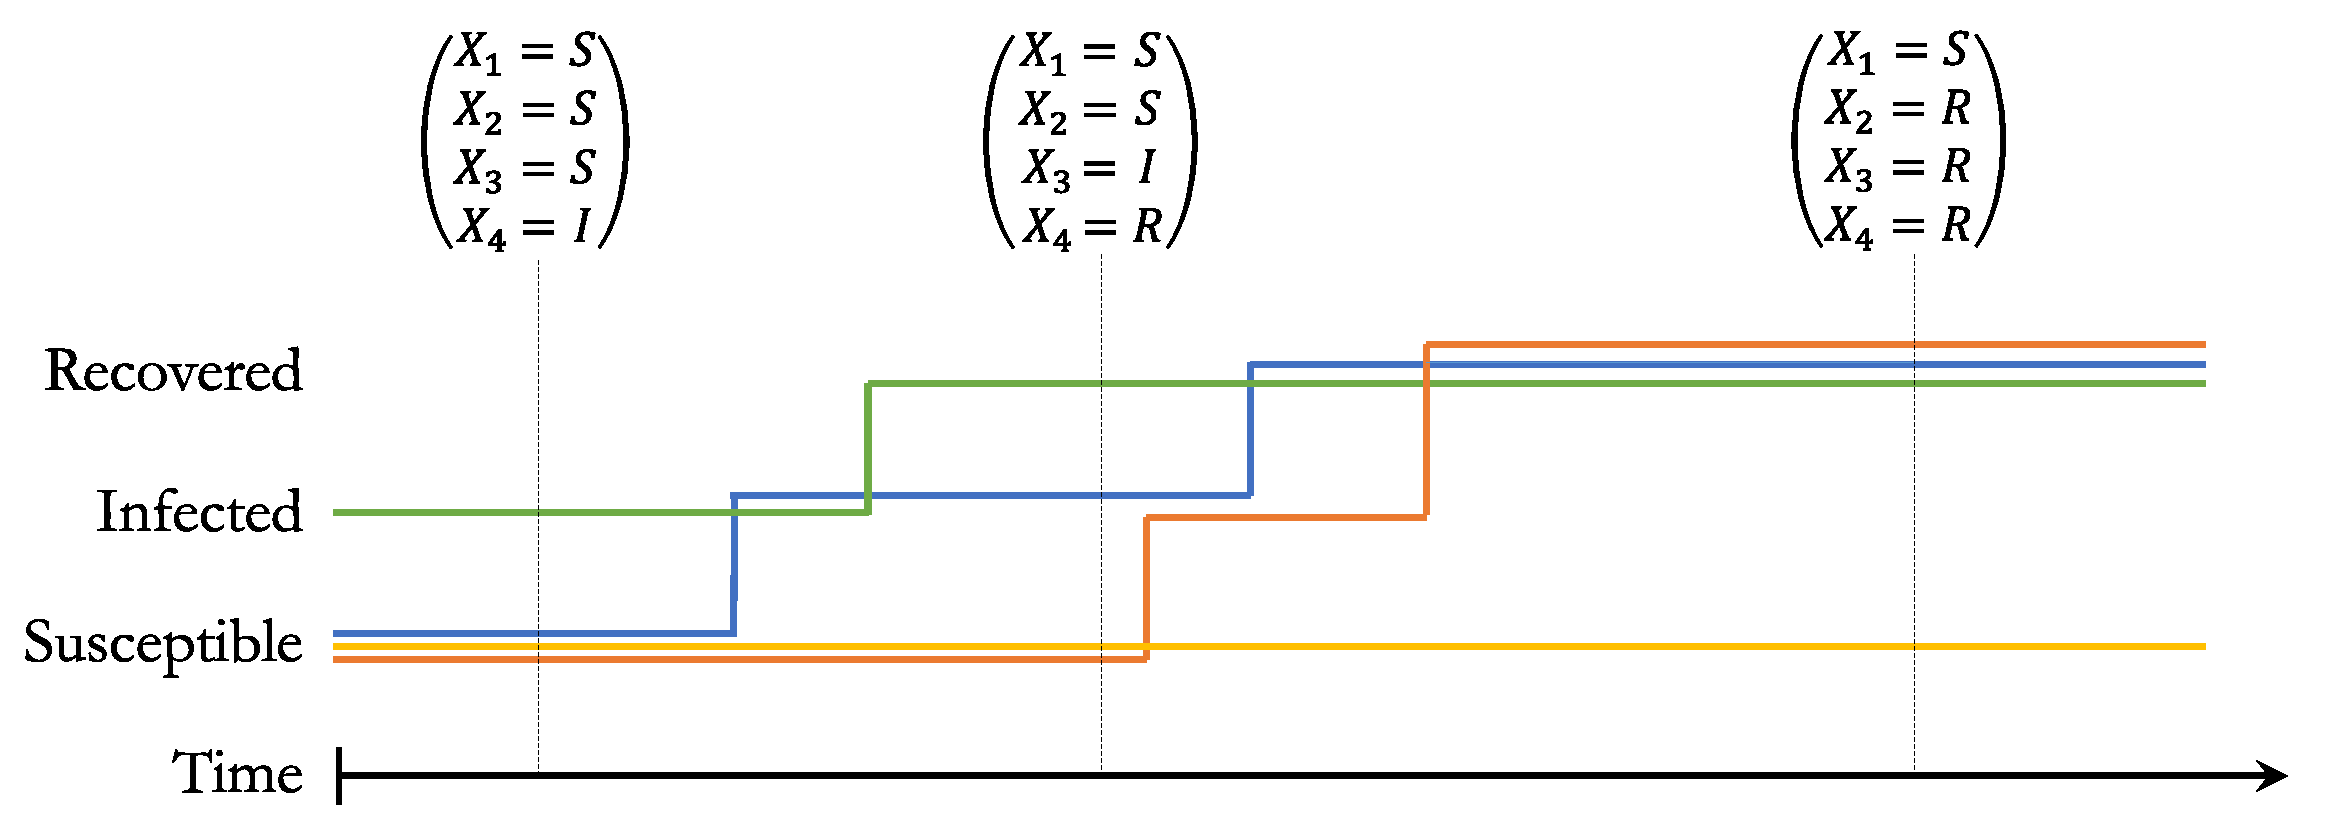
\includegraphics[width=0.8\linewidth]{figures/subject_sample_paths}
	\caption{Diagram of subject--level paths (colored lines) for an SIR model in a population of size $ N=4 $. Individuals transition through infection states continuously in time. The epidemic process is defined in terms of the infection states of individuals in the population.}
	\label{fig:subjectsamplepaths}
\end{figure}

The waiting times between subject--level transition events are typically taken to be exponentially distributed. The exponential distribution has a number of useful properties, enumerated in List \ref{list:exp_props} (see \cite{wilkinson2011stochastic} for proofs). Implications of this choice. Not particularly limiting b/c refs. Then present likelihood, maybe CTMCs. Follow by lumpability and approximations. 

\begin{figure}[htbp]
	\caption{Very useful properties of exponential random variables.}
	\label{list:exp_props}
	\begin{itemize}
		\item (Memoryless property) If $ Z\sim\mr{Exp}(\lambda)$, then $ \forall t,\dt\geq0 $  we have \begin{equation}
		 \Pr(Z > t+\dt | Z>t) = \Pr(Z>\dt).
		\end{equation}
		\item (Racing exponentials) If $ Z_i\sim\mr{Exp}(\lambda_i),\ i=1,\dots,n $, are independent, then \begin{equation}
		\underset{i}{\mr{min}}(Z_i) \sim \mr{Exp}\left (\lambda = \sum_i\lambda_i\right ).
		\end{equation}
		\item (Index of minimum) If $ Z_i\sim\mr{Exp}(\lambda_i),\ i=1,\dots,n $ are independent then the index of the minimum of $ Z_i $ is a random variable with probability mass function \begin{equation}
		\Pr(k|Z_k = \min(Z_1,\dots,Z_n)) = \frac{\lambda_k}{\sum_j\lambda_j}.
		\end{equation} 
	\end{itemize}
\end{figure}


\subsection{Population--level Models}
\label{subsec:pop_level_models}

\subsection{Deterministic Representations}
\label{subsec:deterministic_models}


\subsection{Large--Population Approximations}
\label{subsec:large_pop_approx}

\subsubsection{Diffusion approximations of Markov jump processes}
\label{subsubsec:diff_approx}

\subsubsection{Linear noise approximation}
\label{subsubsec:lna_background}

\section{Computational Approaches to Fitting Stochastic Epidemic Models}
\label{sec:computational_background}

\section{Bayesian Computation and Markov Chain Monte Carlo}
\label{sec:bayesian_computation}

\subsection{Markov Chain Monte Carlo}
\label{subsec:mcmc}

\subsubsection{Bayesian Data Augmentation}
\label{subsec:data_augmentation}

\subsubsection{Slice sampling}
\label{subsubsec:slice_sampling}

\subsubsection{Elliptical slice sampling}
\label{subsubsec:elliptical_slice_sampling}

\subsubsection{Adaptive multivariate normal slice sampling}
\label{subsubsec:mvn_slice_sampling}